\title{Problem Set I}
\author{
        Ethan Rooney \\
        Department of Physics\\
}
\date{\today}

\documentclass[12pt]{article}
\usepackage{amssymb}
\usepackage{amsmath}
\usepackage{cancel}
\usepackage{graphicx}
\usepackage[margin=1in]{geometry}
\begin{document}
\maketitle

\section{Multiplicity of an Einstein Solid}

Since the particles are distinguishable the number of unique micro states we can be calculated following formula for computing the multiplicity of an Einstein Solid.

\begin{equation}
  \Omega(N,q)=\frac{(q + N - 1)!}{q!}
\end{equation}

\begin{equation}
  \Omega(3,8)=\frac{(10)!}{8!}=90
\end{equation}

\section{Quantum Harmonic Ladder Operators}

\begin{equation}
  \int\Psi^*(a_+\phi)dx=\int\phi(\hat{a}_-\Phi)^*dx
\end{equation}

\begin{equation}
  \int\Psi^*(a_-\phi)dx=\int\phi(\hat{a}_+\Phi)^*dx
\end{equation}

\begin{equation}
  \hat{a}_\pm\hat{a}_\mp\psi_n=(E_n\mp\frac{\hbar\omega}{2})\psi_n
\end{equation}

Let $E_n=(n+\frac{1}{2})\hbar\omega$

\begin{equation}
  \hat{a}_+\hat{a}_-\psi_n=(n)\psi_n
\end{equation}

\begin{equation}
  \hat{a}_-\hat{a}_+\psi_n=(n-1)\psi_n
\end{equation}

\begin{equation}
  \int_{-\infty}^\infty (\hat{a}_-\psi_n)^*(\hat{a}_+\psi_n)dx=\lvert c_n \rvert^2 \cancelto{1}{\int_{-\infty}^\infty\lvert \psi_{n} \rvert} = (n+1)
\end{equation}
\begin{equation}
  \int_{-\infty}^\infty (\hat{a}_+\psi_n)^*(\hat{a}_-\psi_n)dx=\lvert d_n \rvert^2 \cancelto{1}{\int_{-\infty}^\infty\lvert \psi_{n} \rvert} = (n)
\end{equation}

\begin{equation}
  \hat{a}_+\psi_n = \sqrt{n+1}\psi_{n+1}
\end{equation}

\begin{equation}
  \hat{a}_-\psi_n = \sqrt{n}\psi_{n-1}
\end{equation}

\begin{equation}
  A_n = \sqrt{n+1}
\end{equation}

\begin{equation}
  B_n = \sqrt{n} 
\end{equation}

Substitue $E_n=(n+\frac{1}{2})\hbar\omega$ back in to get:

\begin{equation}
  \boxed{A_n = \sqrt{\frac{E_n+1}{\hbar\omega}-\frac{1}{2}} }
\end{equation}

\begin{equation}
  \boxed{ B_n = \sqrt{\frac{E_n}{\hbar\omega}-\frac{1}{2}} }
\end{equation}

Relied heavily on Griffiths Into to QM Pg 44-46.

\section{Bound Dirac Delta Well}

Assumptions $lim_{x\to\pm\infty}\Psi(x)=0$, $V(x\neq{0})=0$
 
Starting from Schrodinger's Equation:

\begin{equation}
  \frac{\hbar}{2m}\frac{d^2\Psi}{dx^2}=E\Psi
\end{equation}

\begin{equation}
  \frac{d^2\Psi}{dx^2}=k^2\Psi
\end{equation}

Where $k=\frac{-2mE}{\hbar}$ since $E<0$ $k$ will be real in the following general solution.

\begin{equation}
  \Psi(x)=Ae^{-kx}+Be^{kx}
\end{equation}

When we apply the Boundary Conditions at $\pm\infty$ we find:

For $x\to-\infty$

\begin{equation}
  \Psi(x)=A\cancelto{\infty}{e^{-kx}}+Be^{kx}
\end{equation}

$\Rightarrow A=0$ to keep the equation from blowing up.
And for $x\to\infty$

\begin{equation}
  \Psi(x)=A{e^{-kx}}+B\cancelto{\infty}{e^{kx}}
\end{equation}

\begin{equation}\label{eq:discont}
    \Psi'(0)_{x>0} - \Psi'(0)_{x<0} = lim_{\epsilon\to{}0} \int_\epsilon^\epsilon{}\frac{2m}{\hbar}(V(x)-E)\Psi(x)dx\\
\end{equation}

\begin{equation}
  Bk\cancelto{1}{e^{kx}}-Ak\cancelto{1}{e^{kx}}=\frac{-2ma}{\hbar^2}\Psi(0)
\end{equation}

Since $\Psi(x)$ is continuous at $\Psi(0)$:

\begin{equation}
  \Psi(0)=A\cancelto{1}{e^{-k0}}=B\cancelto{1}{e^{k0}}
\end{equation}


\begin{equation}
  \cancel{B}k+\cancel{B}k=\frac{-2ma}{\hbar^2}\cancel{B}
\end{equation}

Given that $k=\frac{ma}{\hbar^2}=-\frac{2mE}{\hbar}$
\begin{equation}
  \Psi(x)=
    \begin{cases}
      Be^{\frac{max}{\hbar^2}} &\mbox{for } x<0 \\
      Be^{-\frac{max}{\hbar^2}} &\mbox{for } x<0
    \end{cases}
\end{equation}

To find $B$ we can leverage the fact the the partical must be between $-\infty$ and $\infty$.

\begin{equation}
  \int_{-\infty}^{\infty}\Psi^*\Psi=1
\end{equation}

\begin{equation}
  \int_{-\infty}^{O} B^2e^{\frac{2max}{\hbar}} + \int_{0}^{\infty} B^2e^{\frac{-2max}{\hbar}}  = 1
\end{equation}

Because the function is symmetric about the y-axis:


\begin{equation}
  2\int_{0}^{\infty} B^2e^{\frac{-2max}{\hbar}} dx = 1
\end{equation}

\begin{equation}
  \int_{0}^{\infty} B^2e^{\frac{-2max}{\hbar}} dx = \frac{1}{2}
\end{equation}

\begin{equation}
  \cancelto{0}{\int B^2e^{\frac{-2max}{\hbar}}dx}{\rvert}_\infty - {\int B^2e^{\frac{-2max}{\hbar}}dx}{\rvert}_0  = \frac{1}{2}
\end{equation}

\begin{equation}
  \frac{B^2\hbar}{2ma}\cancelto{1}{e^{\frac{-2max}{\hbar}}dx{\rvert}_0}  = \frac{1}{2}
\end{equation}

\begin{equation}
  B=\frac{\sqrt{ma}}{\hbar}
\end{equation}

\begin{equation}
\boxed{
  \Psi(x)=
    \begin{cases}
      \frac{\sqrt{ma}}{\hbar}e^{\frac{max}{\hbar^2}} &\mbox{for } x<0 \\
      \frac{\sqrt{ma}}{\hbar} &\mbox{for } x=0 \\
      \frac{\sqrt{ma}}{\hbar}e^{-\frac{max}{\hbar^2}} &\mbox{for } x<0
    \end{cases}
  }
\end{equation}


\section{Positive Energy Particle with a $-a\delta$ Well}

Given:
\[
  V_x=-a\delta(x)\\
\]
\[
  \Psi(x)=
  \begin{cases}
    e^{ikx}+Ae^{-ikx} &\mbox{for } x<0\\
    Be^{ikx} &\mbox{for } x>0
  \end{cases}
\]

\begin{equation}
  \Psi(0)\rvert_{x<0}=\Psi(0)\rvert_{x>0}
\end{equation}

\begin{equation}
    \cancelto{1}{e^{ikx}\rvert_{x=0}} + A\cancelto{1}{e^{-ikx}\rvert_{x=0}} =B\cancelto{1}{e^{-ikx}\rvert_{x=0}} 
\end{equation}

\begin{equation}
  1+A=B
\end{equation}

From P.3 we can use \eqref{eq:discont} to get:

\begin{equation}
  ik\cancelto{1}{e^{ikx}\rvert_{0}}+-Aik\cancelto{1}{e^{-ikx}\rvert_0}-Bik\cancelto{1}{e^{ikx}\rvert_0}=\frac{2ma}{\hbar^2}\Psi(0)=B\cancelto{1}{e^{ikx}\rvert_0}
\end{equation}

Introduce $\beta=\frac{ma}{\hbar^2k}$

\begin{equation}\label{eq:sub2}
  i(1-A-B)=2\beta(B)
\end{equation}

Given that $R=A^*A$, $T=B^*B$ and $R+T=1$, and $1+A=B$:

\begin{equation}\label{eq:sub}
  \begin{split}
    1+A-2&=B-2\\
    A-1&=B-2
  \end{split}
\end{equation}

Substituting \eqref{eq:sub} into \eqref{eq:sub2}

\begin{equation}
  i(\cancel2-\cancel2B)=\cancel2\beta{}B
\end{equation}

\begin{equation}
  B=\frac{1}{1-i\beta}
\end{equation}

\begin{equation}
  A=\frac{-i\beta}{1-i\beta}
\end{equation}

In Terms of Energy:

\begin{equation}
  A=\frac{-i \frac{a}{\hbar{}2E} }{1-i \frac{a}{\hbar{}2E} }
\end{equation}

\begin{figure}
  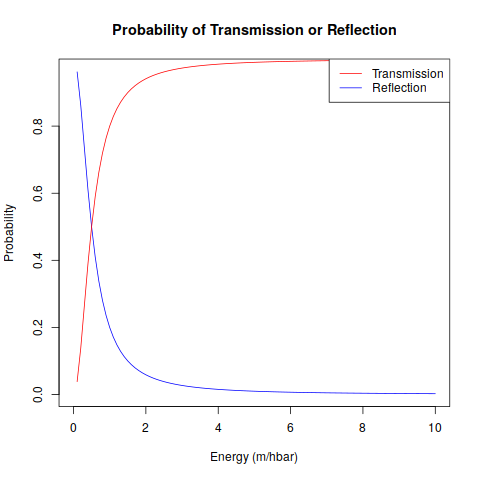
\includegraphics{transorref.png}
  \caption{The Probability of a Reflection Decreases as the Energy of the incoming wave goes up. $a \mbox{ and } \hbar=1$}
\end{figure}



\pagebreak
\section{Computational}

First turn the Schr{\"o}dinger Equation into a system of first order differential equations:

\begin{verbatim}
void f( double complex* vect, double complex* res , double x, double energy)
{
  res[1] = k(x, energy)*cexp(I*k(x, energy)*x);
  res[0] = vect[1]; //dx/dt = v_x
}
\end{verbatim}

Next this was used in an rk2 integrator function from $x=1$ to $x=0$. This should have given me the value of $\Psi(0)$
\begin{verbatim}
    while ( x > 0 )
    {
      integrate_rk2(Psi, dx, Psin, x, e);
      x -= dx;
      Psi[0] = Psin[0];
      Psi[1] = Psin[1];
    }
\end{verbatim}

Then once The value of $\Psi$ was determined I could use that to determine the value of $B$ and then determine the value of the transmission and reflection at various energies. Which could then be plotted. It seems the code I wrote expects the probability of reflection to converge at 50\%. That seems none physical.

\begin{figure}
  \centering
  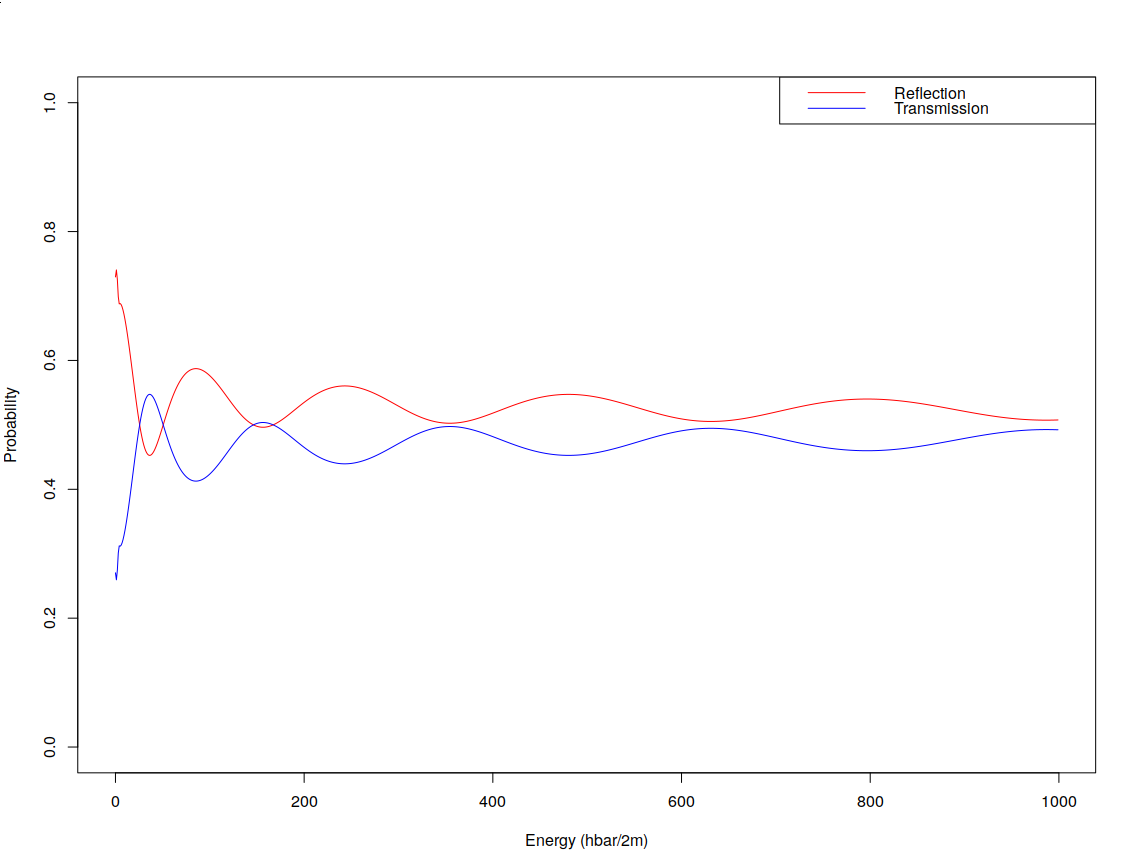
\includegraphics[width=500pt]{bounce.png}
  \caption{I think I made an Error somewhere as I would expect the Transmission Probability trend up as Energy Increases.}
\end{figure}



\end{document}

